\documentclass{ufscThesis}

\usepackage[brazil]{babel}
%o outro tipo de encoding geralmente usado no windows é o "ansinew"
\usepackage[utf8]{inputenc}

\usepackage{amsmath}
\usepackage{indentfirst}
\usepackage{multirow}
\usepackage{graphicx}
\usepackage{float}
\usepackage{circuitikz}
\usepackage{pgfplots}
\pgfplotsset{compat=1.8}

\usepackage{rotating}
\usepackage{tikz-timing}
\usepackage{listings}
\usepackage{color}
\lstset{language=C,frame=single}
\usepackage{makeidx}
\makeindex

\titulo{Uma nova abordagem para a troca de
       lâmpadas elétricas: utilizando um banquinho}
\autor{Ramiro Polla}
\data{18}{abril}{2013}

\orientador{Prof. Dr. Fulano}                    % Nome do orientador e (opcional) seu título
\coorientador{Prof. Dr. Beltrano}                % Nome do coorientador e seu título (opcional)
\coordenador{Prof. Chefe, Dr. Eng.}              % Nome do coordenador do curso e (opcional) seu título

%\departamento[a]{Faculdade de Ciências do Mar}
%\curso[a]{Atividade de Extensão em Corte e Costura}


%%% Sobre a Banca
\numerodemembrosnabanca{5} % Isso decide se haverá uma folha adicional
\orientadornabanca{sim} % Se faz parte da banca definir como sim
\coorientadornabanca{sim} % Se faz parte da banca definir como sim
\bancaMembroA{Prof. Presidente da banca} %Nome do presidente da banca
\bancaMembroB{Prof. segundo membro}      % Nome do membro da Banca
\bancaMembroC{Prof. terceiro membro}     % Nome do membro da Banca
\bancaMembroD{Prof. quarto membro}       % Nome do membro da Banca
\bancaMembroE{Prof. quinto membro}       % Nome do membro da Banca
\bancaMembroF{Prof. sexto membro}        % Nome do membro da Banca
\bancaMembroG{Prof. sétimo membro}       % Nome do membro da Banca

\dedicatoria{A quem o trabalho é dedicado, se é que o é (opcional)}

\agradecimento{Agradecimentos opcionais, caso existam pessoas ou entidades a quem se deve apoio ou suporte ao trabalho ora apresentado.}

\epigrafe{Um bonito pensamento ou citação, se for o caso}{autor do pensamento}

\textoResumo {Aqui é redigido o resumo do documento...  blabla blablablabla blabla ipsum loren e a sophia também blab ablablabl ablbalbalblab lablablbalb lab lab lab labl a blab lablablab la blab alballbalba lba lba }

\palavrasChave {chave 1. chave 2. ... chave n.}

\textAbstract {Here is written the abstract of the document}

\keywords {key 1. key 2. ... key n.}

\newcommand{\vetor}[1]{\textbf{#1}}

\hyphenation{a-b-c-d-e-f-g-h-i-j-k-l-m-n-o-pq-rs-tu-vw-xy-za-b-c-de-fg-hi-jk-l-m-n-op-qr-st-uv-w-x-yz}

\begin{document}

\capa  
\folhaderosto[comficha] % Se nao quiser imprimir a ficha, é só não usar o parâmetro
\folhaaprovacao
\paginadedicatoria
\paginaagradecimento
\paginaepigrafe
\paginaresumo
\paginaabstract
\listadefiguras
\listadetabelas 
\listadeabreviaturas
\sumario

\chapter{Introdução}
\label{sec:intro}

As lâmpadas elétricas são amplamente utilizadas nos dias
de hoje para a iluminação residencial.
Em geral, tais lâmpadas estão dispostas no teto dos cômodos,
longe do alcance de pessoas de estatura mediana.

% http://www.igf.min-financas.pt/inflegal/bd_igf/bd_legis_geral/leg_geral_docs/dl_650_75.htm
O pé-direito 
\footnote{pé direito se define como a distância entre o pavimento e o teto}
das construções tem valor mínimo de 2,40 metros e valor máximo de 2,70 metros.

% http://www.ibge.gov.br/home/estatistica/populacao/condicaodevida/pof/2008_2009_encaa/tabelas_pdf/tab1_1.pdf
A tabela \ref{tab:ibge} mostra alguns dos dados das estimativas populacionais das
medianas de altura e peso do povo brasileiro por sexo.

\begin{table}[!htb]
  	\centering
  	\begin{tabular}{|l|r|r|}
  	\hline
    \multirow{2}{*}{Faixa etária} & \multicolumn{2}{|c|}{Altura (cm)} \\ \cline{2-3}
                 & Masculino & Feminino \\ \hline
    18      anos & 172,6 & 161,1 \\
    19      anos & 172,0 & 161,2 \\
    20 a 24 anos & 173,0 & 161,1 \\
    25 a 29 anos & 173,0 & 160,7 \\
    30 a 35 anos & 171,6 & 160,0 \\
    \hline
    \end{tabular}
    \label{tab:ibge}
\end{table}

% Nossos estudos mostraram que um homem com o braço esticado alcança 1.35 vezes sua altura
% amostragem: 1 pessoa, eu mesmo. mascarar isso de algum jeito pra parecer mais sério
Considerando que um homem com o braço esticado alcança 1.35 vezes sua altura,
podemos dizer que um homem na faixa etária de 20 a 24 anos alcança 2.34 metros,
o que chega perto, porém ainda alguns centímetros a menos, do valor mínimo do
pé-direito residencial.
Para as mulheres, o problema é maior. Sua altura com o braço esticado alcança
2.13 metros, muito aquém do mínimo do pé-direito residencial.

O estado da arte em troca de lâmpadas nas ocasiões em que não se é possível
alcança-la meramente esticando-se o braço envolve subir nos ombros de um parceiro,
conforme a Figura \ref{fig:ombros}.

% http://loscaneros.blogspot.com.br/2012/07/quantas-pessoas-sao-nescessarias-para.html
\begin{figure}[!htb]
  \centering
  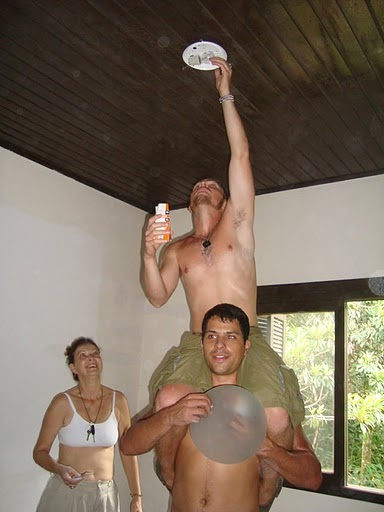
\includegraphics[width=0.5\textwidth]{ombros.jpg}
  \caption{Trocando lâmpada subindo nos ombros de um parceiro}
  \label{fig:ombros}
\end{figure}


Neste trabalho iremos apresentar uma nova abordagem
para a troca de lâmpadas elétricas:
subindo num banquinho. % hehehe

% aqui eu tenho que melhorar a introducao

\chapter{A lâmpada elétrica}
\label{sec:alampada}

Existem vários tipos de lâmpadas elétricas:
\begin{itemize}
\item Incandescente;
\item Fluorescente;
\item de Vapor de Sódio;
\item entre outras. % péssima ideia, não coloque isso no seu TCC
\end{itemize}

O símbolo elétrico utilizado para a lâmpada incandescente está
exposto na Figura \ref{fig:simbolo_lampada}.

\begin{figure}[!htb]
\centering
\begin{tikzpicture}
\draw (0,0) to[lamp] (2,0);
\end{tikzpicture}
\caption{Símbolo elétrico da lâmpada incandescente}
\label{fig:simbolo_lampada}
\end{figure}

\chapter{O banquinho}
\label{sec:banquinho}

Nos primórdios da humanidade, os seres humanos sentavam-se em
pedras, troncos de árvore, ou até mesmo montinhos de terra.
Com o passar do tempo, o ser humano passou a ser mais civilizado
e passou a fabricar ferramentas que o ajudassem no dia-a-dia.

Para sentar, o ser humano inventou um dispositivo revolucionário
chamado o \emph{banquinho} (vide Figura \ref{fig:banquinho}).

\begin{figure}[!htb]
  \centering
  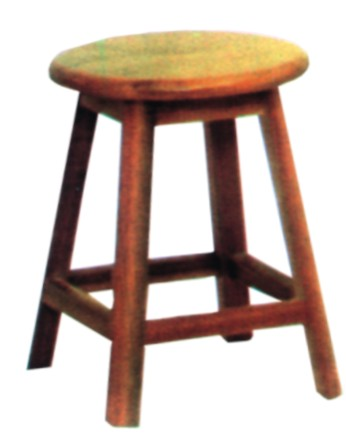
\includegraphics[width=0.5\textwidth]{banquinho.jpg}
  \caption{O banquinho}
  \label{fig:banquinho}
\end{figure}

%http://br.answers.yahoo.com/question/index?qid=20091125150826AA7YDiN
De acordo com fontes confiáveis (a segunda resposta de uma pergunta
no \textit{Yahoo! Answers}), o tamanho ideal de um banquinho hoje em
dia é de 60 a 70~cm.


\chapter{Motivação}
\label{sec:motiv}

Pessoas muito baixas não conseguem trocar lâmpadas.
O presente trabalho sugere que elas subam num
banquinho para alcançar a lâmpada.

\hfill

Como vimos na introducao (secao \ref{chap:intro}, página \pageref{chap:intro}),
...

\begin{quotation}
Money, que é good, nóis num have.
Se nóis hevasse, nóis num tava aqui playando
Mas nóis precisa de worká.
Money, que é good, nóis num have.
Se nóis hevasse, nóis num tava aqui workando.
O nosso work é playá.
\end{quotation}

Uma fórmula qualquer: $V=R I$

$$I = \frac{V}{R}$$

$$0=1+e^{j\pi}$$

IDFT (fórmula numero \ref{eq:idft}):

\begin{equation}
\label{eq:idft}
x_n = \frac{1}{N}
\sum_{k=0}^{N-1} X_k \cdot
e^{i2\pi kn/N}
\end{equation}

Equacoes de maxwell (\ref{eq:max1} e \ref{eq:max2}).

\begin{align}
\label{eq:max1}
\nabla \cdot \vetor{E} & = \frac{\rho}{\epsilon_0} \\
\label{eq:max2}
\nabla \cdot \vetor{B} & = 0 \\
\nabla \times \vetor{E}
& = - \frac{\partial \vetor{B}}{\partial t} \\
\nabla \times \vetor{B} & =
\mu_0\vetor{J} + \mu_0 \epsilon_0
\frac{\partial \vetor{E}}{\partial t}
\end{align}

\begin{figure}
 \begin{center}
 \begin{sideways}
  \begin{tikztimingtable}
   clk & 20{C} \\
   $\overline{\text{cs}}$  & HHHLLLHHHLLLHLTTTTTT \\
  \end{tikztimingtable}
 \end{sideways}
 \end{center}
\end{figure}

Vamos fazer uma referência ao livro do \emph{Franklin} \cite{franklin}.

Inclinando-se para a esquerda faz a torre Eiffel parecer menor: \cite{eerland2011leaning}.

a b c d abcdefghijklmnopqrstuvwxyzabcdefghijklmnopqrstuvwxyz e f g.

\printindex

\bibliography{tcc}
\bibliographystyle{plain}

\anexo
\chapter{Código}
\begin{lstlisting}
#include <stdio.h>
int main(int argc, char *argv[])
{
	printf("Hello!\n");
    return 0;
}
\end{lstlisting}

\end{document}